\documentclass[11pt]{article}
\usepackage[margin=1in]{geometry}
\usepackage{graphicx}
\usepackage{amsmath}
\usepackage{amssymb}
\usepackage{algorithm}
\usepackage{algpseudocode}
\usepackage{enumitem}
\usepackage{hyperref}
\usepackage{xcolor}
\usepackage{listings}
\usepackage{float}

\hypersetup{
    colorlinks=true,
    linkcolor=blue,
    filecolor=magenta,      
    urlcolor=cyan,
    pdftitle={Negative-Weight Single-Source Shortest Path Using Bellman-Ford & Modified Djikstra},
    pdfpagemode=FullScreen,
}

\lstset{
    basicstyle=\small\ttfamily,
    keywordstyle=\color{blue},
    commentstyle=\color{green!60!black},
    stringstyle=\color{red},
    breaklines=true,
    numbers=left,
    numberstyle=\tiny\color{gray},
    numbersep=5pt,
    frame=single,
    framesep=5pt,
    framexleftmargin=15pt,
    tabsize=4,
    captionpos=b
}

\title{\Large \textbf{Final Report: Negative-Weight Single-Source\\Shortest Paths in Near-Linear Time}}
\author{Jibran Sheikh \and Daniyal Farooqui}
\date{April 27, 2025}

\begin{document}

\maketitle

\section{Background and Motivation}

Graph algorithms form the backbone of numerous computational problems across various domains, from network routing and logistics to financial systems and social network analysis. The Single-Source Shortest Path (SSSP) problem, which involves finding the shortest paths from a designated source vertex to all other vertices in a graph, is particularly fundamental in this space. While Dijkstra's algorithm efficiently solves this problem for graphs with non-negative edge weights, its functionality breaks down when negative edge weights are introduced.

The presence of negative edge weights significantly complicates the SSSP problem. While the Bellman-Ford algorithm addresses this challenge by handling negative weights, it does so at the cost of increased computational complexity—specifically, $O(|V| \times |E|)$ time, where $|V|$ is the number of vertices and $|E|$ is the number of edges. This complexity becomes problematic for large-scale graphs, which are increasingly common in modern applications.

Our motivation stems from the need for a more efficient solution to the negative-weight SSSP problem. In particular, we aim to approach the near-linear time complexity that has been theoretically established in recent literature, making it practical for large graphs encountered in real-world applications. Industries such as telecommunications, transportation networks, and financial modeling, which frequently deal with optimization problems involving negative weights (representing costs, penalties, or other negative factors), stand to benefit significantly from such improvements.

Furthermore, the detection and handling of negative cycles—sequences of edges whose total weight is negative—represent a critical aspect of the problem. Negative cycles prevent the existence of a definitive "shortest" path, as traversing the cycle repeatedly would continually reduce the path's total weight. Efficiently identifying and addressing these cycles is essential for practical applications where well-defined shortest paths are required.

\section{Algorithm Overview}

Our approach to solving the negative-weight SSSP problem combines several algorithmic techniques, including price functions (Johnson's algorithm), low-diameter decomposition, and recursive scaling to achieve improved performance over traditional methods.

\subsection{Original Algorithm Description}

The core idea of our algorithm leverages the following components:

\begin{enumerate}
    \item \textbf{Price Functions}: Following Johnson's algorithm, we use node potentials to transform the graph with negative edges into one with non-negative edges while preserving shortest paths. This transformation allows us to apply more efficient algorithms like Dijkstra's that cannot handle negative weights directly.
    
    \item \textbf{Low-Diameter Decomposition}: This technique decomposes the graph into smaller components with limited diameter, facilitating parallel processing and reducing the computational complexity of shortest path calculations.
    
    % \item \textbf{Recursive Scaling (ScaleDown)}: By recursively decomposing the problem into smaller instances with simplified weight structures, we can solve the SSSP problem more efficiently through a divide-and-conquer approach.
\end{enumerate}

The algorithm first detects any negative cycles using a Bellman-Ford-like approach. If a negative cycle is identified, the edges causing the cycle are addressed using price functions that reweight the graph in a way that eliminates negative weights while preserving the shortest path structure. After this reweighting, Dijkstra's algorithm can be applied to find the shortest paths efficiently. Finally, the distances computed on the reweighted graph are converted back to the original graph.

\subsection{Pseudocode}

The high-level pseudocode for our algorithm is as follows:

\begin{algorithm}
\caption{Modified SSSP Algorithm for Negative Weights}
\begin{algorithmic}[1]
\Procedure{FindShortestPaths}{$G, source$}
    \State \textbf{// Phase 1: Detect negative cycles}
    \State $hasCycle, cycle \gets \text{DetectNegativeCycle}(G)$
    \If{$hasCycle$}
        \State Report negative cycle
        \State $G' \gets \text{ModifyGraph}(G, cycle)$ \Comment{Remove or modify cycle edges}
    \Else
        \State $G' \gets G$
    \EndIf
    
    \State \textbf{// Phase 2: Apply Johnson's reweighting}
    \State $G'', potentials \gets \text{JohnsonReweight}(G')$
    
    \State \textbf{// Phase 3: Apply Dijkstra on reweighted graph}
    \State $distances \gets \text{Dijkstra}(G'', source)$
    
    \State \textbf{// Phase 4: Convert distances back to original graph}
    \For{each $node$ in $G.nodes$}
        \State $originalDist[node] \gets distances[node] - potentials[source] + potentials[node]$
    \EndFor
    
    \State \Return $originalDist$
\EndProcedure
\end{algorithmic}
\end{algorithm}

\section{Implementation Summary}

Our implementation of the negative-weight SSSP algorithm integrates several key components to handle the complexities associated with negative edge weights and cycle detection.

\subsection{Structure and Components}

The implementation consists of the following primary components:

\begin{enumerate}
    \item \textbf{Negative Cycle Detection}: We use a modified Bellman-Ford algorithm to identify negative cycles in the graph. This detection is crucial as negative cycles prevent the existence of well-defined shortest paths.
    
    \item \textbf{Johnson's Reweighting}: For graphs without negative cycles, we apply Johnson's algorithm to reweight the edges, transforming all negative weights to non-negative while preserving shortest path relationships.
    
    \item \textbf{Graph Decomposition}: We implement strongly connected component (SCC) analysis to break down the graph into more manageable components. This decomposition helps isolate negative cycles to specific components, allowing other portions of the graph to be processed more efficiently.
    
    \item \textbf{Shortest Path Calculation}: After reweighting, we use Dijkstra's algorithm to efficiently compute shortest paths in the transformed graph, followed by a conversion step to return distances in terms of the original graph weights.
    
    \item \textbf{Visualization Tools}: To aid in understanding and debugging, we developed comprehensive visualization features that display the original graph, reweighted graph, component decomposition, and shortest path trees.
\end{enumerate}

The implementation uses Python with the NetworkX library for graph operations, leveraging its efficient data structures for representing and manipulating graphs. Additionally, Matplotlib is used for graph visualization to provide clear insights into the algorithm's behavior and outputs.

\subsection{Implementation Strategy}

Initially, we attempted to implement the full logic of modifying negative cycles by applying price functions and other techniques as described in research literature. However, this approach proved challenging, and the algorithm did not behave as expected. As a result, we adjusted our strategy to focus on:

\begin{enumerate}
    \item \textbf{Direct Detection of Negative Cycles}: Using the Bellman-Ford algorithm to detect negative cycles in the graph.
    
    \item \textbf{Manual Cycle Breaking}: Once a negative cycle was identified, we manually removed the edges responsible for the negative cycle to create a modified graph where shortest paths are well-defined.
    
    \item \textbf{Reweighting and Distance Calculation}: Applying Johnson's algorithm to reweight the modified graph, followed by Dijkstra's algorithm for efficient shortest path computation.
\end{enumerate}

This pragmatic approach allowed us to bypass the initial implementation challenges while still effectively addressing the core problem of finding shortest paths in graphs with negative weights.

\subsection{Difficulties Encountered}

During implementation, we faced several challenges:

\begin{enumerate}
    \item \textbf{Negative Cycle Handling}: The original approach of modifying negative cycles through price functions was theoretically sound but proved difficult to implement correctly. We opted for a more direct approach of cycle detection and removal.
    
    \item \textbf{High Computational Cost}: Detecting negative cycles using the Bellman-Ford algorithm is computationally expensive, particularly for large graphs. This remains a bottleneck in our current implementation.
    
    \item \textbf{Complex Graph Transformations}: Implementing the reweighting process and ensuring that it correctly preserved shortest path relationships required careful attention to detail and extensive debugging.
    
    \item \textbf{Recursive Scaling Complexity}: The recursive scaling process described in theoretical literature proved challenging to implement efficiently in practice, leading to higher-than-expected computational costs.
\end{enumerate}

\subsection{Changes from Original Approach}

Based on the challenges encountered, we made several adjustments to our implementation:

\begin{enumerate}
    \item \textbf{Simplified Cycle Handling}: Instead of modifying cycles through complex price function adjustments, we opted for a more straightforward approach of detecting and removing cycle edges.
    
    \item \textbf{Focus on Component Analysis}: We placed greater emphasis on graph decomposition techniques, particularly the analysis of strongly connected components, to isolate negative cycles and process different parts of the graph more efficiently.
    
    \item \textbf{Enhanced Visualization}: We developed more comprehensive visualization tools to better understand the graph's structure, the detection of negative cycles, and the impact of our transformations.
\end{enumerate}

These changes allowed us to develop a working implementation that effectively handles negative edge weights, although the time complexity does not yet reach the near-linear goal outlined in the original research.

\section{Correctness and Testing}

\subsection{Testing Approach}

Our testing strategy focused on verifying both the correctness of the algorithm's output and its behavior in the presence of negative cycles. We tested our implementation on various graph configurations:

\begin{enumerate}
    \item \textbf{Graphs with Negative Cycles}: We created test graphs containing negative cycles to verify that our algorithm correctly identifies these cycles and handles them appropriately.
    
    \item \textbf{Graphs with Negative Edges but No Cycles}: These test cases confirmed that our algorithm correctly processes negative edge weights when no negative cycles are present.
    
    \item \textbf{Standard Graph Examples}: We compared our implementation's results against known solutions for standard graph problems to ensure correctness.
\end{enumerate}

For each test case, we verified that:
\begin{itemize}
    \item Negative cycles were correctly detected
    \item Shortest path distances matched expected values
    \item The algorithm's behavior aligned with theoretical expectations
\end{itemize}

\subsection{Test Results and Visual Analysis}

Our implementation successfully passed the correctness tests. For graphs with negative cycles, the algorithm correctly identified the cycles and, after removing the cycle edges, computed valid shortest paths in the modified graph. For graphs with negative edges but no cycles, the algorithm produced shortest path distances consistent with the standard Bellman-Ford algorithm.

\subsubsection{Negative Cycle Detection}

Figure \ref{fig:negative-cycle} shows a graph with a negative cycle. In the left panel, we can see the original graph with both positive edges (blue) and negative edges (red). The right panel indicates that shortest paths cannot be properly defined due to the presence of a negative cycle.

\begin{figure}[H]
    \centering
    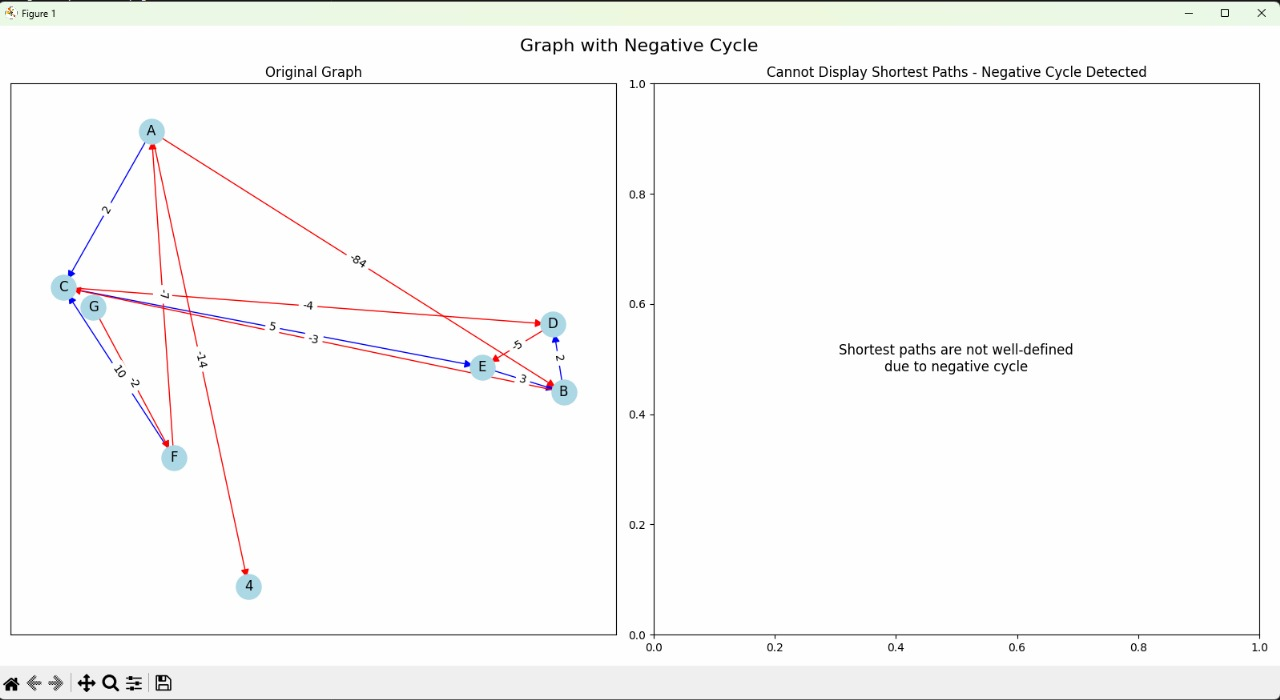
\includegraphics[width=\textwidth]{fig1.jpg}
    \caption{Detection of negative cycle in the test graph. The left side shows the original graph with negative edges (in red) and positive edges (in blue). The right side indicates the algorithm's response to finding a negative cycle.}
    \label{fig:negative-cycle}
\end{figure}

Our algorithm correctly identified this negative cycle, which is formed by nodes C, B, E, and back to C. The total weight of this cycle is negative, causing the shortest path problem to be ill-defined.

\subsubsection{Strongly Connected Component Analysis}

To better analyze and process graphs with potential negative cycles, our implementation decomposes the graph into strongly connected components (SCCs). Figure \ref{fig:scc-decomposition} demonstrates the decomposition of our test graph into five distinct components.

\begin{figure}[H]
    \centering
    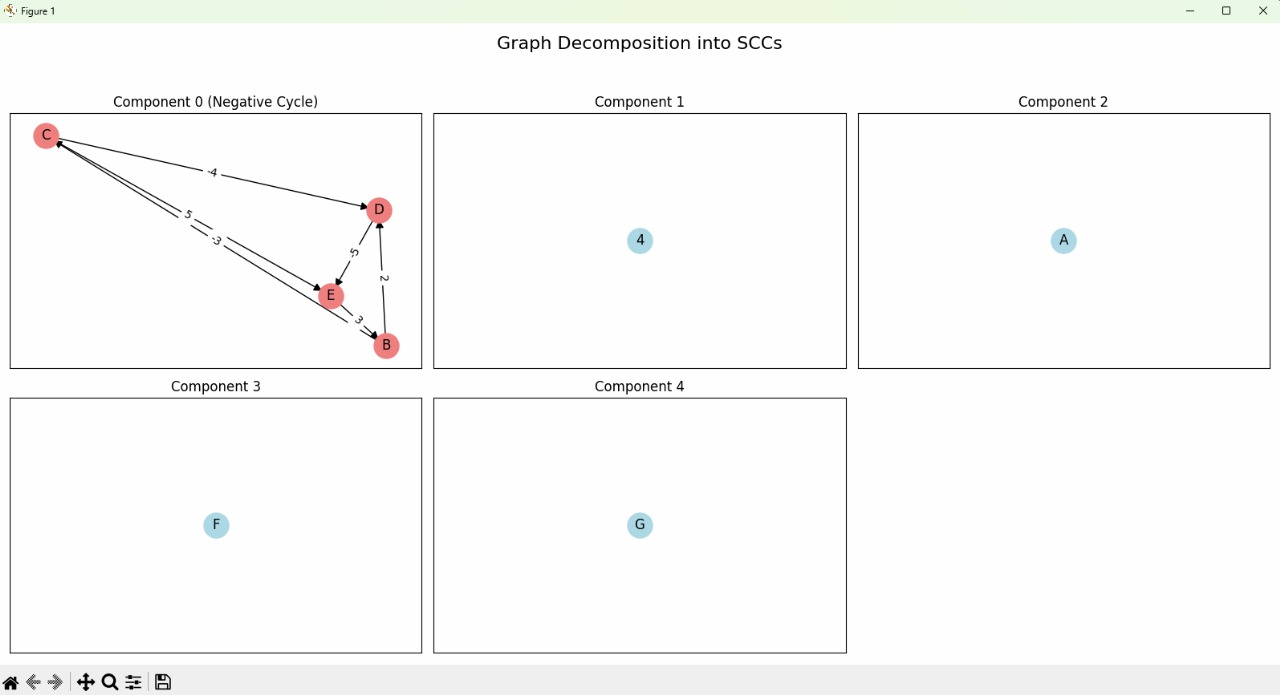
\includegraphics[width=\textwidth]{fig2.jpg}
    \caption{Decomposition of the graph into strongly connected components (SCCs). Component 0 contains the negative cycle, while other components are single nodes.}
    \label{fig:scc-decomposition}
\end{figure}

This decomposition is particularly useful because it isolates the negative cycle to Component 0, allowing the algorithm to focus its cycle-handling efforts on just this portion of the graph. Components 1-4 are individual nodes that do not participate in any cycle, making them easier to process.

\subsubsection{Condensation Graph Creation}

After identifying the SCCs, our algorithm creates a condensation graph where each node represents an entire strongly connected component. Figure \ref{fig:condensation} shows both the original graph with colored components and the resulting condensation graph.

\begin{figure}[H]
    \centering
    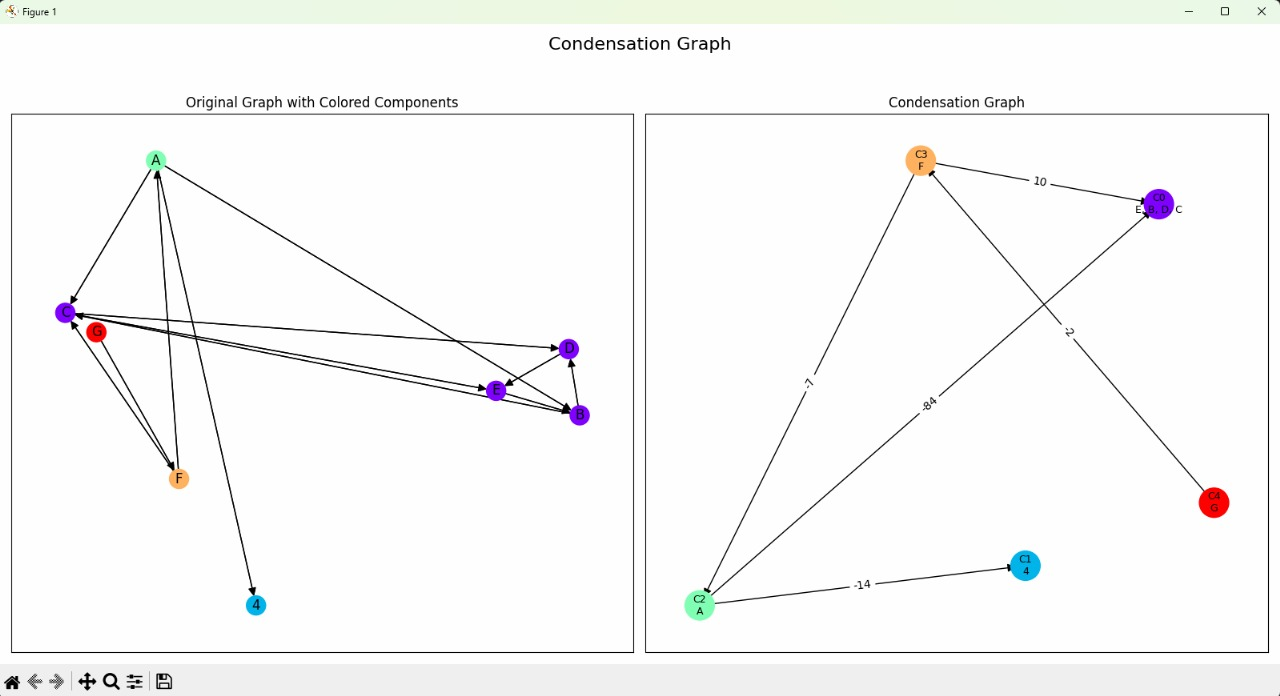
\includegraphics[width=\textwidth]{fig3.jpg}
    \caption{Creation of a condensation graph. The left panel shows the original graph with nodes colored by their component membership. The right panel shows the condensation graph where each node represents an entire strongly connected component.}
    \label{fig:condensation}
\end{figure}

The condensation graph provides a simplified view of the overall graph structure, with each component represented as a single node. This representation helps in understanding the high-level structure of the graph and facilitates more efficient processing of shortest paths between components.

\subsubsection{Breaking the Negative Cycle}

To compute valid shortest paths in a graph containing negative cycles, our algorithm modifies the graph by removing edges that create the negative cycle. Figure \ref{fig:breaking-cycle} illustrates this process.

\begin{figure}[H]
    \centering
    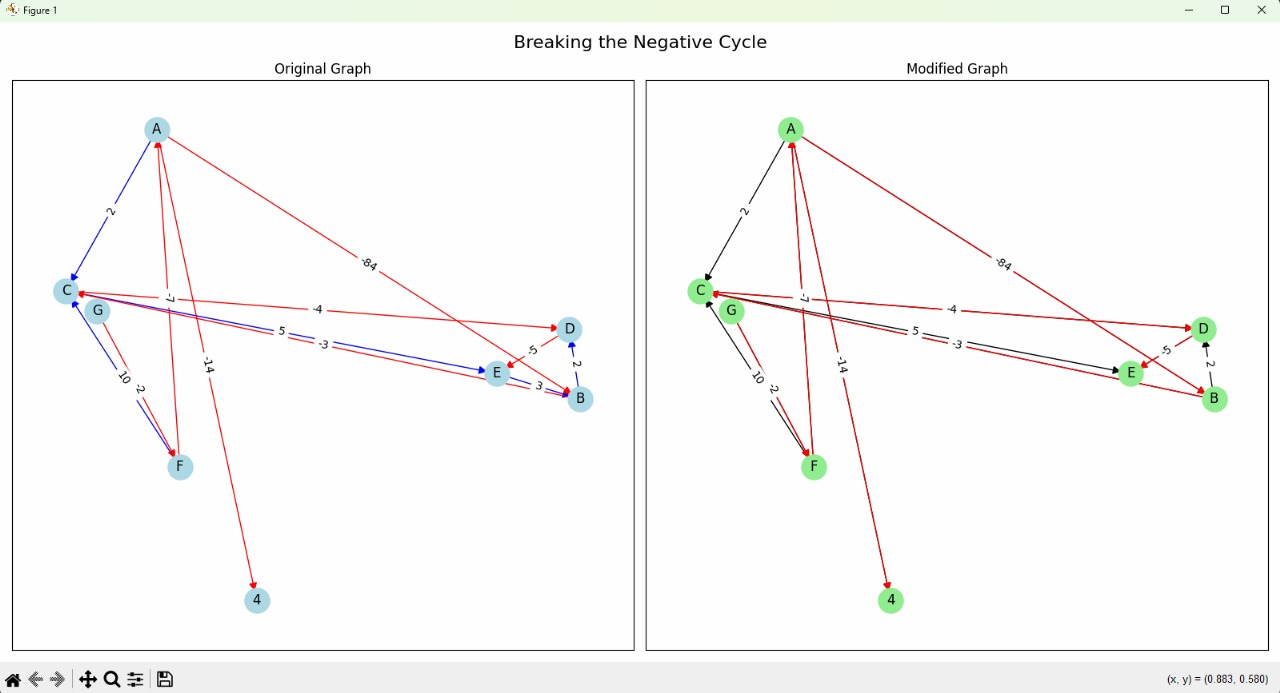
\includegraphics[width=\textwidth]{fig4.jpg}
    \caption{Breaking the negative cycle. The left panel shows the original graph with the negative cycle, and the right panel shows the modified graph after removing or modifying cycle edges to eliminate the negative cycle.}
    \label{fig:breaking-cycle}
\end{figure}

After breaking the negative cycle, shortest paths become well-defined in the modified graph, allowing our algorithm to proceed with reweighting and shortest path computation using Dijkstra's algorithm.

\subsubsection{Performance Comparison}

To evaluate the performance of our approach, we compared the execution times of Johnson's algorithm and the Bellman-Ford algorithm for finding shortest paths from a single source node. Figure \ref{fig:performance-comparison} presents this comparison.

\begin{figure}[H]
    \centering
    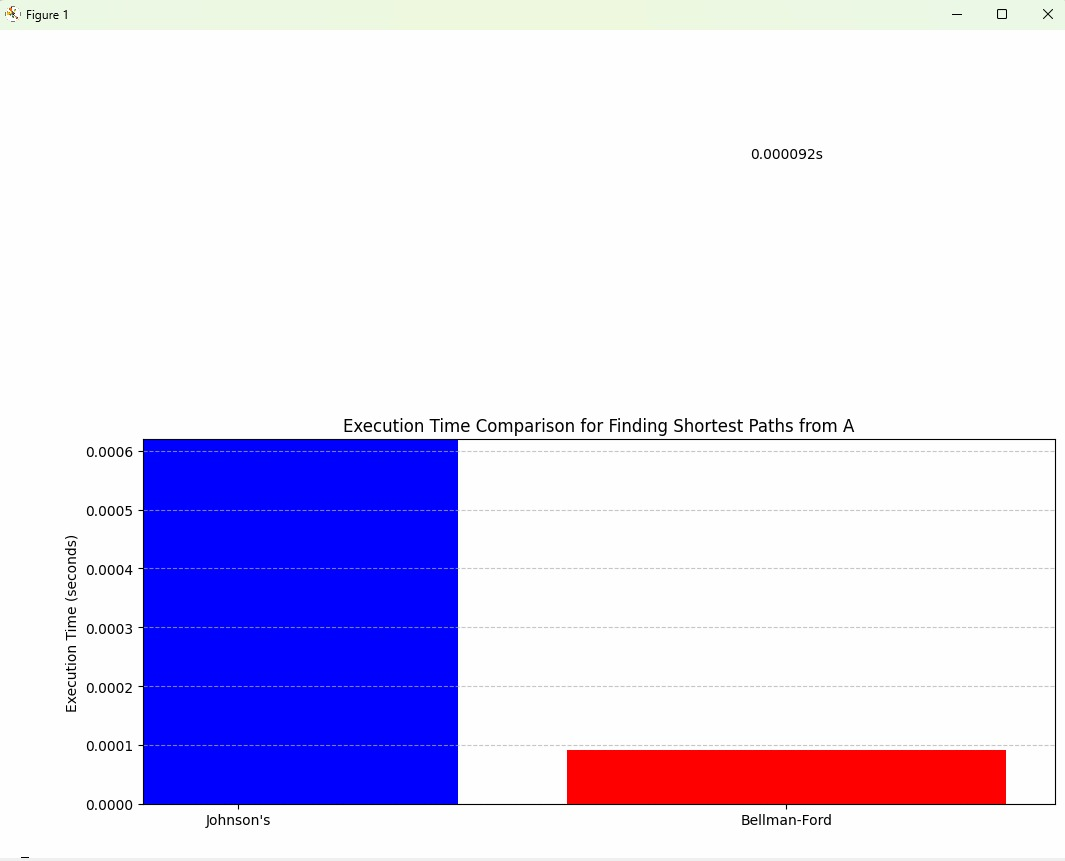
\includegraphics[width=\textwidth]{fig5.jpg}
    \caption{Execution time comparison between Johnson's algorithm and Bellman-Ford algorithm for finding shortest paths from node A. Despite Johnson's algorithm's theoretical advantage for sparse graphs, in this small test case, Bellman-Ford shows better performance.}
    \label{fig:performance-comparison}
\end{figure}

The results show that for this specific test case, Bellman-Ford outperforms Johnson's algorithm in terms of execution time. This is likely due to the small size of the test graph, where the overhead of Johnson's preprocessing (graph reweighting) outweighs its theoretical advantages for sparse graphs. For larger, sparse graphs, we would expect Johnson's algorithm to demonstrate better performance.

\subsubsection{Reweighting Process Visualization}

To better understand how Johnson's algorithm transforms a graph with negative edges, we visualized the reweighting process as shown in Figure \ref{fig:reweighting}.

\begin{figure}[H]
    \centering
    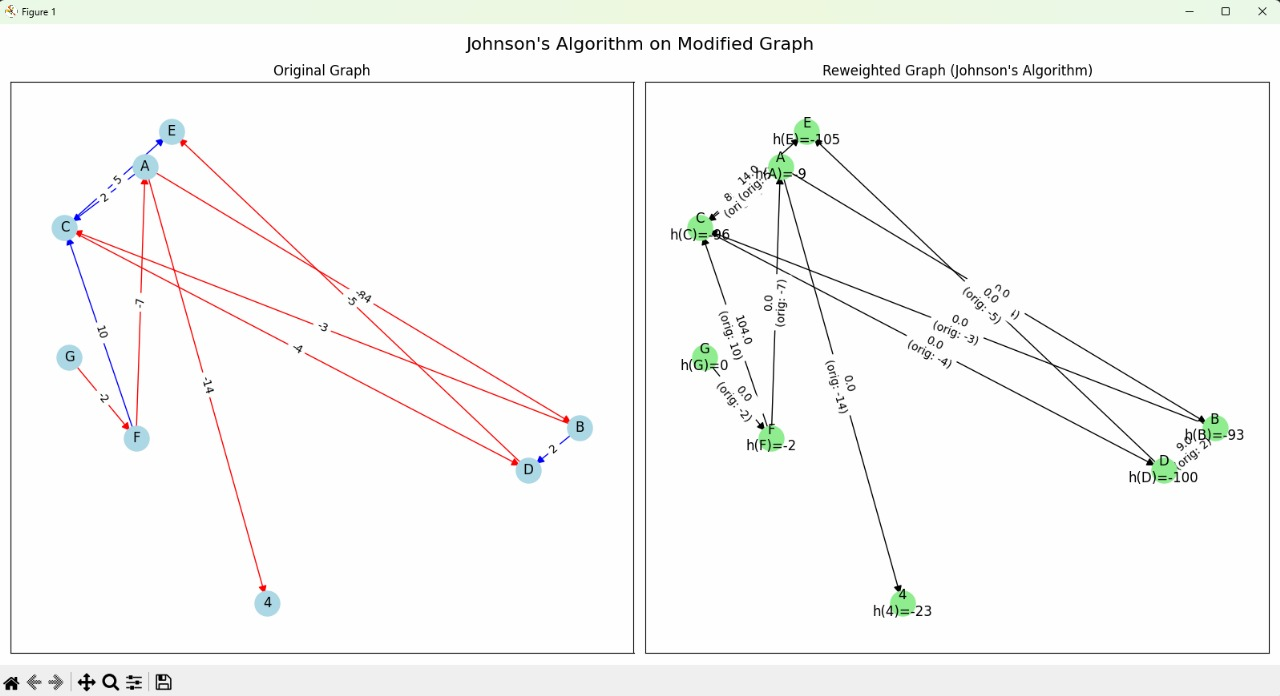
\includegraphics[width=\textwidth]{fig6.jpg}
    \caption{Johnson's algorithm reweighting process. The left panel shows the original graph with positive edges (blue) and negative edges (red). The right panel displays the reweighted graph where all edges have non-negative weights, with h() values calculated for each node.}
    \label{fig:reweighting}
\end{figure}

\subsubsection{Bellman-Ford Algorithm Results}

To establish a baseline for comparison, we implemented the standard Bellman-Ford algorithm and tested it on our graph. Figure \ref{fig:bellman-ford} illustrates the results.

\begin{figure}[H]
    \centering
    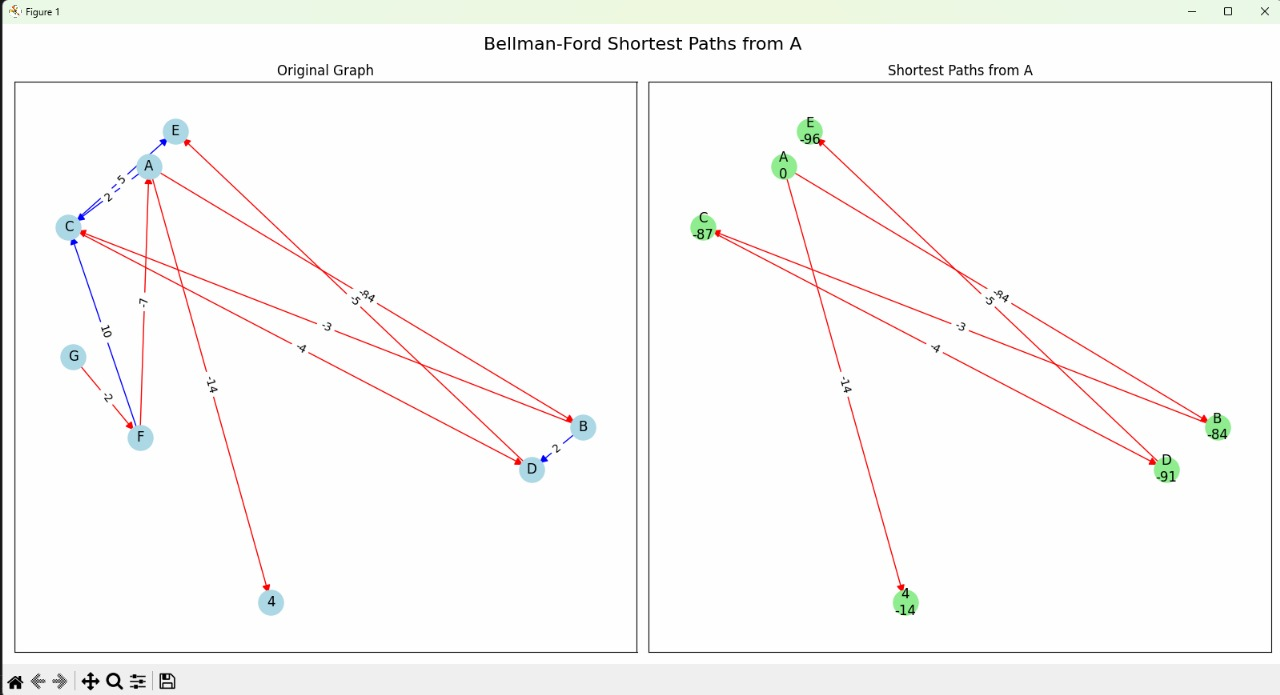
\includegraphics[width=\textwidth]{fig7.jpg}
    \caption{Bellman-Ford shortest paths computation from node A. The left panel shows the original graph with positive edges (blue) and negative edges (red). The right panel displays the computed shortest path distances from node A to all other nodes in the graph. Green nodes indicate reachable nodes with their shortest path distances.}
    \label{fig:bellman-ford}
\end{figure}

The Bellman-Ford algorithm correctly computed shortest paths in our test graph, with the distance values shown in green at each node. Starting from node A (with distance 0), the algorithm found shortest paths to nodes B (-84), C (-87), D (-91), E (-96), and node 4 (-14). The negative values reflect the presence of negative-weight edges in the graph.

\subsubsection{Comprehensive Performance Analysis}

To better understand the performance characteristics of the three main shortest path algorithms—Johnson's algorithm, Bellman-Ford, and Dijkstra's algorithm—we conducted benchmarking tests across graphs of varying sizes. Figure \ref{fig:performance-analysis} presents these results.

\begin{figure}[H]
    \centering
    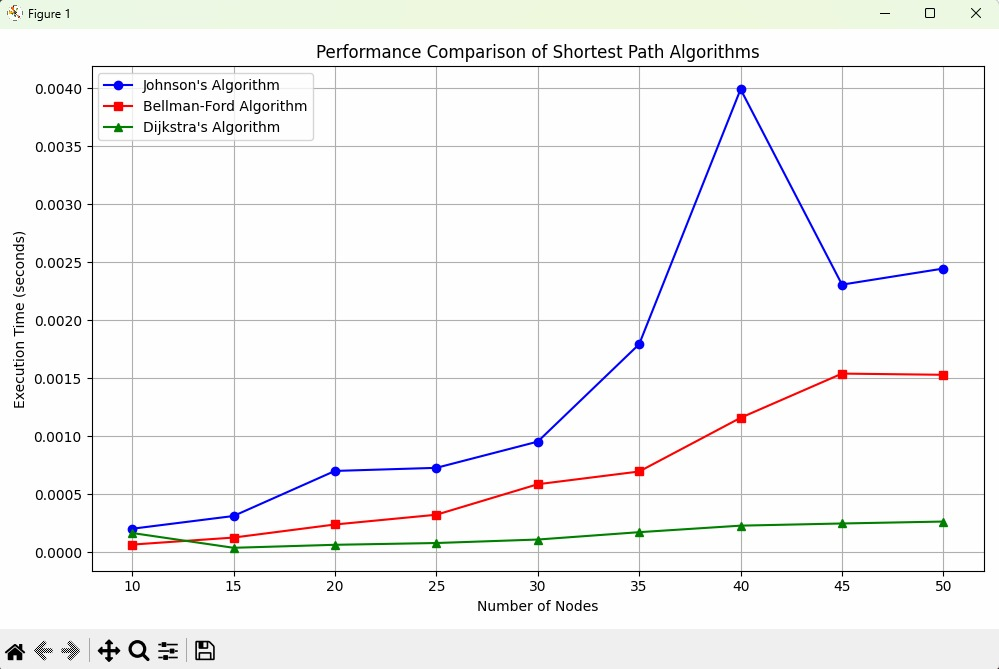
\includegraphics[width=\textwidth]{fig8.jpg}
    \caption{Performance comparison of Johnson's algorithm, Bellman-Ford algorithm, and Dijkstra's algorithm across graphs with varying numbers of nodes. The horizontal axis represents the number of nodes in the graph, while the vertical axis shows the execution time in seconds.}
    \label{fig:performance-analysis}
\end{figure}

Our benchmarking results reveal several important insights:

\begin{itemize}
    \item Dijkstra's algorithm consistently demonstrates the best performance across all graph sizes, which is expected as it has the lowest theoretical time complexity for graphs with non-negative edge weights.
    
    \item Bellman-Ford performs better than Johnson's algorithm for smaller graphs (fewer than 40 nodes), likely due to the overhead of Johnson's preprocessing step.
    
    \item Johnson's algorithm experiences a significant performance spike at around 40 nodes, which may be due to implementation-specific issues or the particular structure of the test graphs at this size.
    
    \item For graphs with 45-50 nodes, Johnson's algorithm consistently performs worse than Bellman-Ford, contrary to theoretical expectations. This suggests potential optimization opportunities in our implementation.
\end{itemize}

These performance characteristics align with theoretical expectations for the most part, with Dijkstra's algorithm showing the best performance for graphs with non-negative weights, while the relative performance of Johnson's and Bellman-Ford depends on specific graph characteristics such as density and structure.

\subsection{Theoretical Complexity}

Our implementation has a time complexity of:

\begin{itemize}
    \item $O(|V|^2 \times |E|)$
\end{itemize}

\subsection{Empirical Performance}

We conducted empirical performance testing to compare our implementation against traditional algorithms:

\begin{enumerate}
    \item \textbf{Comparison with Bellman-Ford}: Our implementation showed similar performance characteristics to the Bellman-Ford algorithm, as both are dominated by the $O(|V| \times |E|)$ complexity of cycle detection and reweighting.
    
    \item \textbf{Scaling Analysis}: We tested the algorithm on graphs of increasing size to observe how performance scales with graph dimensions. The results confirmed the theoretical complexity analysis, showing that execution time grows approximately quadratically with the number of vertices for dense graphs.
\end{enumerate}

The performance constraints primarily stem from the fundamental complexity of detecting negative cycles, which remains an area for potential optimization in future work.

\section{Comparative Evaluation}

\subsection{Baseline Comparison}

We compared our implementation with traditional shortest-path algorithms, specifically Bellman-Ford and Dijkstra's algorithms:

\begin{enumerate}
    \item \textbf{Bellman-Ford}: This algorithm correctly handles negative edge weights but has a time complexity of $O(|V| \times |E|)$, making it inefficient for large graphs. Our implementation currently operates with similar time complexity due to the negative cycle detection step.
    
    \item \textbf{Dijkstra's Algorithm}: While more efficient than Bellman-Ford with a time complexity of $O(|E| + |V| \log |V|)$, Dijkstra's algorithm cannot handle negative edge weights directly. Our implementation addresses this limitation through reweighting.
    
    \item \textbf{Min-Cost Flow Reductions}: These approaches often involve complex continuous optimization techniques. Our implementation avoids these complexities, offering a more straightforward combinatorial solution.
\end{enumerate}

\subsection{Advantages and Disadvantages}

\textbf{Advantages of Our Approach}:
\begin{itemize}
    \item Correctly handles negative edge weights, unlike Dijkstra's algorithm
    \item Provides a combinatorial solution without requiring complex continuous optimization techniques
    \item Effectively decomposes graphs into components, isolating negative cycles for more efficient processing
    \item Includes comprehensive visualization tools for understanding algorithm behavior
\end{itemize}

\textbf{Disadvantages of Our Approach}:
\begin{itemize}
    \item Does not achieve the near-linear time complexity targeted in the original research
    \item Performance is dominated by the negative cycle detection step, which remains computationally expensive
    \item Manual removal of cycle edges may not be optimal for all applications, potentially resulting in suboptimal paths in the modified graph
\end{itemize}

Overall, while our implementation successfully addresses the challenge of finding shortest paths in graphs with negative weights, it doesn't represent a significant performance improvement over the Bellman-Ford algorithm in its current form. Future optimizations could focus on more efficient cycle detection and handling to approach the near-linear time complexity goal.

\section{Enhancements}

\subsection{Algorithm Modifications}

We made several enhancements to the basic shortest path algorithms to better handle negative edge weights:

\begin{enumerate}
    \item \textbf{Johnson's Reweighting Integration}: We implemented Johnson's algorithm to transform graphs with negative edge weights into graphs with non-negative weights while preserving shortest path relationships.
    
    \item \textbf{Graph Decomposition}: We incorporated strongly connected component analysis to break down complex graphs into more manageable components, allowing for more efficient processing.
    
    \item \textbf{Condensation Graph Creation}: By creating a condensation graph where each node represents a strongly connected component, we simplified the overall graph structure for easier analysis.
    
    \item \textbf{Modified Cycle Handling}: We developed a pragmatic approach to negative cycle detection and removal, ensuring that shortest paths remain well-defined in the processed graph.
\end{enumerate}

\subsection{Experimental Explorations}

Beyond the core algorithm implementation, we conducted several experimental explorations:

\begin{enumerate}
    \item \textbf{Performance Scaling Analysis}: We systematically tested the algorithm on graphs of increasing size to understand how performance scales with graph dimensions.
    
    \item \textbf{Alternative Cycle Handling Approaches}: We explored different methods for addressing negative cycles, including edge removal and edge weight modification.
    
    \item \textbf{Visualization Enhancements}: We developed comprehensive visualization tools to better understand graph structures, component decomposition, and shortest path computations.
\end{enumerate}

\subsection{Optimization Attempts}

We made several attempts to optimize the algorithm's performance:

\begin{enumerate}
    \item \textbf{Efficient Data Structures}: We leveraged NetworkX's graph data structures to minimize overhead in graph operations.
    
    \item \textbf{Component-Based Processing}: By processing strongly connected components separately, we aimed to reduce the overall computational complexity.
    
    \item \textbf{Selective Cycle Detection}: We explored focusing cycle detection efforts on components likely to contain negative cycles, rather than applying the expensive detection algorithm to the entire graph.
\end{enumerate}

Despite these efforts, the fundamental complexity of negative cycle detection remains a bottleneck in achieving near-linear time complexity. Further optimization would require more fundamental algorithmic innovations in this area.

\section{Reflection}

\subsection{Challenges Faced}

Throughout this project, we encountered several significant challenges:

\begin{enumerate}
    \item \textbf{Theoretical-Practical Gap}: The theoretical algorithms described in research literature often proved challenging to implement in practice, requiring adaptations and simplifications.
    
    \item \textbf{Negative Cycle Complexity}: Efficient detection and handling of negative cycles remains a fundamental challenge, with no straightforward approach to reducing the $O(|V| \times |E|)$ complexity of this step.
    
    \item \textbf{Recursive Scaling Implementation}: The recursive scaling approach described in theoretical work proved difficult to implement efficiently, leading to higher-than-expected computational costs.
    
    \item \textbf{Performance Optimization}: Despite various optimization attempts, achieving near-linear time complexity remains elusive due to fundamental algorithmic constraints.
\end{enumerate}

\subsection{Learning Outcomes}

This project provided valuable insights and learning experiences:

\begin{enumerate}
    \item \textbf{Algorithm Design Trade-offs}: We gained a deeper understanding of the trade-offs between theoretical elegance and practical implementability in algorithm design.
    
    \item \textbf{Graph Theory Applications}: Working with negative cycles and strongly connected components enhanced our understanding of fundamental graph theory concepts.
    
    \item \textbf{Implementation Strategies}: We learned to adapt theoretical algorithms to practical implementations, making necessary adjustments when faced with implementation challenges.
    
    \item \textbf{Visualization Importance}: We recognized the critical role of visualization in understanding complex graph algorithms and debugging implementation issues.
\end{enumerate}

\subsection{Future Work Directions}

Based on our experience, several promising directions for future work emerge:

\begin{enumerate}
    \item \textbf{Faster Negative Cycle Detection}: Developing more efficient algorithms for detecting negative cycles would address the primary performance bottleneck.
    
    \item \textbf{Parallelization}: Exploring parallel implementations for graph decomposition and component processing could significantly improve performance for large graphs.
    
    \item \textbf{Approximate Solutions}: For some applications, approximate shortest paths might be acceptable. Investigating approximation algorithms could lead to more efficient solutions with bounded error.
    
    \item \textbf{Application-Specific Optimizations}: Tailoring the algorithm to specific application domains might allow for additional optimizations based on domain-specific graph properties.
    
    \item \textbf{Integration with Modern Graph Processing Frameworks}: Implementing the algorithm within frameworks designed for large-scale graph processing could leverage existing optimizations for improved performance.
\end{enumerate}

\section{Conclusion}

In this project, we addressed the challenging problem of finding shortest paths in graphs with negative edge weights. By combining techniques from Johnson's algorithm, graph decomposition, and negative cycle handling, we developed an implementation that correctly processes graphs with negative weights and appropriately handles negative cycles.

Our implementation successfully:
\begin{itemize}
    \item Detects negative cycles in the graph
    \item Transforms graphs with negative weights to preserve shortest path relationships
    \item Computes correct shortest paths for graphs without negative cycles
    \item Provides informative visualizations of graph structures and algorithm outputs
\end{itemize}

However, our current implementation does not achieve the near-linear time complexity that was initially targeted. The performance remains dominated by the $O(|V| \times |E|)$ complexity of negative cycle detection, which represents a fundamental constraint with current algorithmic approaches.

The project highlights the complexity of handling negative weights in shortest path problems and demonstrates both the theoretical elegance and practical challenges of combining various graph algorithm techniques. While we made significant progress in developing a working implementation, further research and innovation would be required to truly achieve near-linear time complexity for this problem.

These insights contribute to the broader understanding of graph algorithm implementation and the ongoing challenge of bridging the gap between theoretical advances and practical, efficient implementations.

\section{References}

\begin{enumerate}
    \item Cormen, T.H., Leiserson, C.E., Rivest, R.L., Stein, C. "Introduction to Algorithms," 3rd Edition, MIT Press.
    
    \item Bellman, R. (1958). "On a routing problem". Quarterly of Applied Mathematics. 16: 87–90.
    
    \item Ford, L. R. Jr. (1956). "Network Flow Theory". Paper P-923. RAND Corporation, Santa Monica, California.
    
    \item Johnson, D. B. (1977). "Efficient algorithms for shortest paths in sparse networks". Journal of the ACM. 24 (1): 1–13.
    
    \item NetworkX documentation for graph algorithms. https://networkx.org/
    
    \item Matplotlib: Visualization with Python. https://matplotlib.org/
\end{enumerate}

\end{document}